\section{プロジェクトの背景,目的,目標}
\label{section:project}

\subsection{背景}

\subsubsection{ゲームを超えたXRへの期待の高まり}

昨今 VR(Virtual Reality)や AR(Augmented Reality)などのXRが世間から注目を浴びている.
IDCの2022年3月のレポート\cite{idc} によると,世界の AR/VR ヘッドセットの市場は2021年で
92.1\% 成長し,1000万台を超えるヘッドセットが出荷された.
また,ヘッドセットの市場は2026年まで年平均35.1\%で成長し,
2026年に出荷されるヘッドセットは5000万台を超えると予想されている(図\ref{fig:idc}).

\begin{figure}[htbp]
  \begin{minipage}[b]{0.50\linewidth}
    \centering
    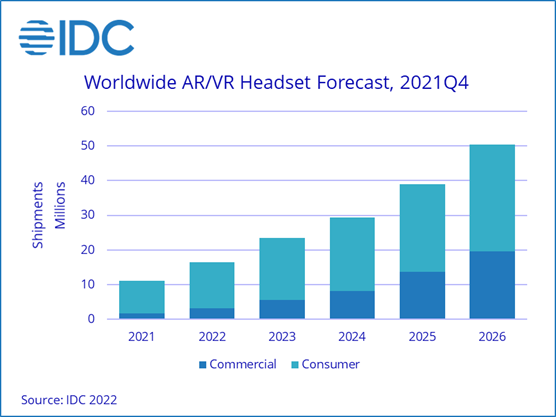
\includegraphics[keepaspectratio, width=0.9\linewidth]{fig/idc.png}
    \caption{IDCによる世界のAR/VRヘッドセットの市場予測}
    \label{fig:idc}
  \end{minipage}
  % \begin{minipage}[b]{0.50\linewidth}
  %   \centering
  %   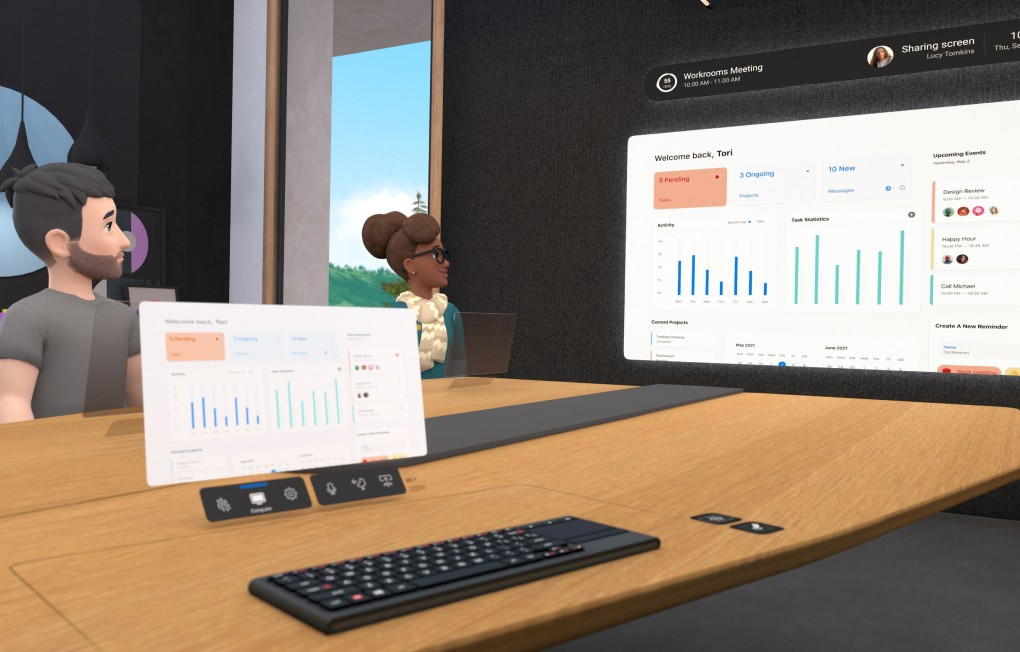
\includegraphics[keepaspectratio, width=0.9\linewidth]{fig/workrooms.jpeg}
  %   \caption{Horizon Workrooms (Meta社)}
  %   \label{fig:workrooms}
  % \end{minipage}
  \begin{minipage}[t]{0.50\linewidth}
    \centering
    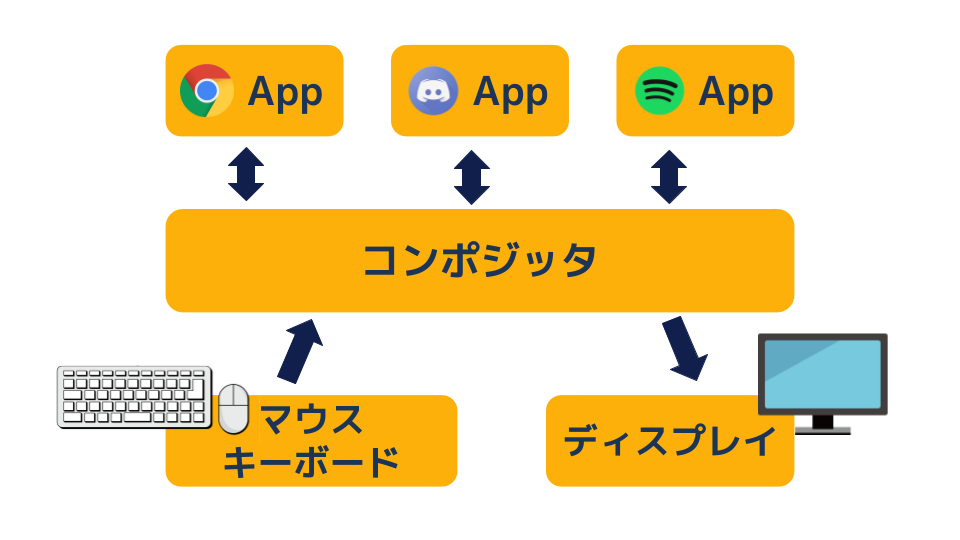
\includegraphics[keepaspectratio, width=\linewidth]{fig/2d-windowing-system.png}
    \caption{2D Windowing Systemの概要図}
    \label{fig:2d-windowing-system}
  \end{minipage}
\end{figure}

特に2021年はメタバースへの期待が高まった年であり,同年10月の Facebook 社の社名変更などから
もうかがえ,XRは従来のゲーム利用を超えた,より幅広い日常生活での利用が期待されている.
Meta社は特に
"Infinite Office\footnote{Infinite Office - Meta Quest:\url{https://www.youtube.com/watch?v=5_bVkbG1ZCo&t=1s}}"
のコンセプトのもと,ビジネス会議用VRアプリ,Horizon Workroom
\footnote{Horizon Workrooms - Meta Quest:\url{https://www.oculus.com/workrooms/}}
(図\ref{fig:workrooms})を発表し,仕事・作業のためのXR空間の重要性が示唆されている.

% コロナ・リモートワークの影響を書いてもいい

\subsubsection{通常の2Dデスクトップ環境におけるWindowing Systemについて}

今日において GUI デスクトップ環境ではWindowing System
(Linuxでは X11やWayland,macOSではQuartz compositorなど)が用いられており,
これによって優れた作業環境を提供できている.
Windowing Systemではアプリケーションが直接自身の描画内容をディスプレイに出力したり,
マウスなどのインプットデバイスからの入力を受け取ったりせず,ディスプレイサーバや
コンポジッタと呼ばれるソフトウェアとのやりとり(プロセス間通信)を介して
これらのハードウェアを扱うようにしている(図\ref{fig:2d-windowing-system}).
コンポジッタの主な役割は,
\begin{itemize}
  \item 複数のアプリケーションから描画内容を受け取り,
        それらを一枚のスクリーンに合成してディスプレイに表示する.
  \item マウスやキーボードなどのハードウェアからの入力を適切なアプリケーション
        (ユーザがフォーカスしているアプリケーションなど)に割り振る.
  \item ドラッグ\&ドロップなどのアプリケーション間のデータ共有の仕組みを提供する.
\end{itemize}
などである.これによって,開発元の異なる複数のアプリケーションを同じディスプレイ上にウィンドウが
自然に重なる形で表示したり,また1つのマウスやキーボードでフォーカスを切り替えながら複数の
アプリケーションを操作したりでき,マルチアプリケーション・マルチタスクの環境が実現されている.

\begin{figure}[htbp]
  \begin{minipage}[t]{0.50\linewidth}
    \centering
    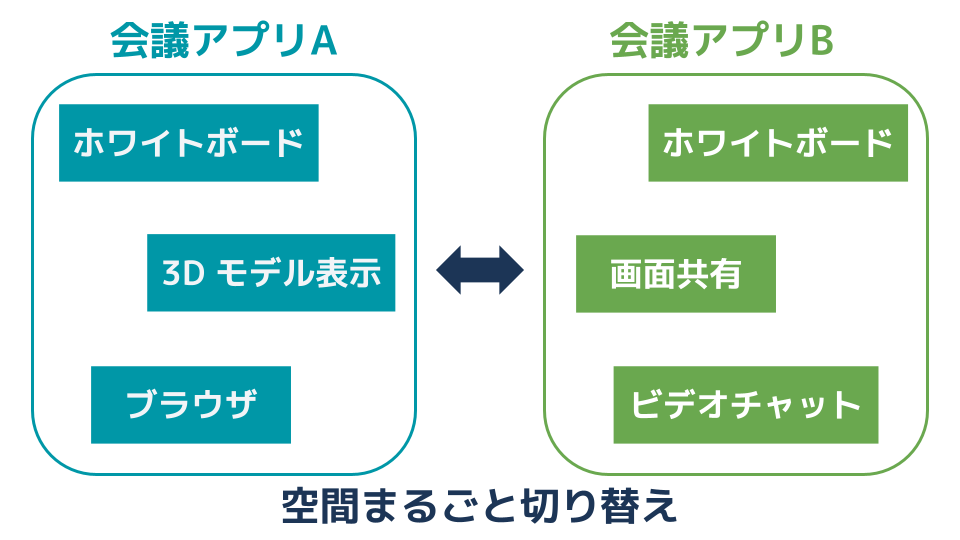
\includegraphics[keepaspectratio, width=0.9\linewidth]{fig/xr-app-switch.png}
    \caption{
      現状のXRアプリケーションの切り替え.アプリケーションの切り替えは,空間内の全ての
      機能を切り替えることになってしまう.
    }
    \label{fig:xr-app-switch}
  \end{minipage}
  \begin{minipage}[t]{0.50\linewidth}
    \centering
    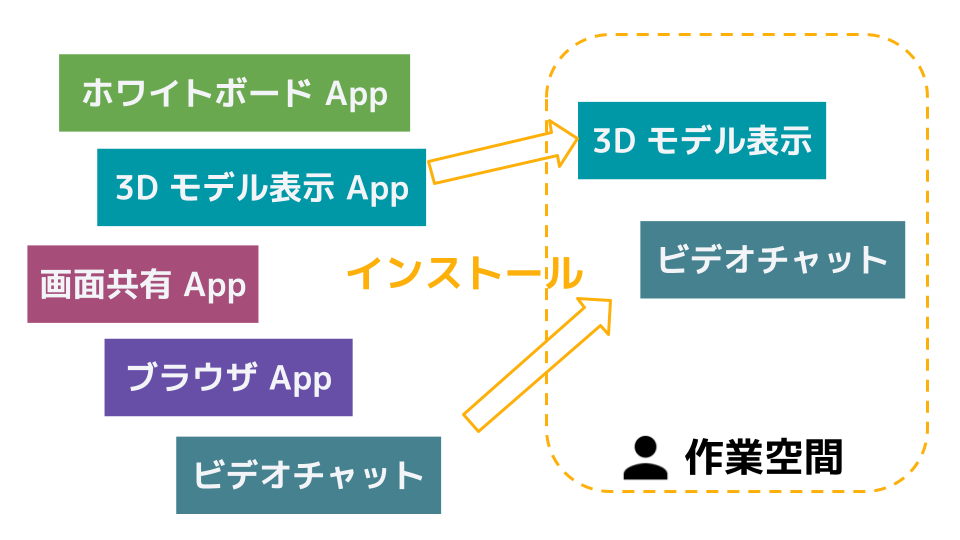
\includegraphics[keepaspectratio, width=\linewidth]{fig/xr-app-install.png}
    \caption{XR空間でユーザが好きなアプリケーションをインストールして同時に複数使う.}
    \label{fig:xr-app-install}
  \end{minipage}
\end{figure}

\subsubsection{現状のXRアプリケーションについて}

2Dのデスクトップ環境では複数のアプリケーションが同時に,連携して使用できるのに対し,
現状のXRアプリケーションは基本的に1つのメインアプリケーションがユーザの視界の全てを支配する.
そのため,アプリケーションを切り替えると,空間ごと切り替えることに
なってしまい(図 \ref{fig:xr-app-switch}),XRアプリケーションは,その空間に必要な
機能をその1つのアプリケーションが全て実装している必要がある.
1つのアプリケーションが1つの世界観を作り出すXRゲームなどにおいてはこれで問題ないが,
作業空間としてXRを用いたい場合は問題が生じる.
作業空間に必要な機能は個人ごとに大きく異なり多様性が大きいため,1つのアプリケーションが
全てのニーズに応えて機能を実装するのは現実的に不可能である.
例えば図\ref{fig:xr-app-switch}の例で,会議アプリAを利用しているユーザが会議アプリBの
画面共有のような機能を3Dモデルの表示と一緒に使いたいと思っても,
それは会議アプリAの開発元が画面共有機能を追加しない限り不可能である.

簡易的に複数のアプリケーションを重ねて表示する機能を提供する仕組みも存在するが,
それについては\ref{section:openxr-overlay}で詳しく言及する.
% また特に,このような汎用的な会議アプリケーションに対して,ニーズの割合が小さい,例えば
% 医療CTスキャンの結果を表示するようなアプリケーションは実装されないだろう.
% そして逆に医療CTスキャンの結果を表示したいモチベーションの開発者が同時に会議アプリケーション
% としての機能を実装することもないと考えられるため,XR会議をしながらCTスキャンの結果を
% 見るという世界が実現する可能性は低い.

\subsubsection{何が必要か}

特に作業空間としてのXRでは,全ての機能を1つのアプリケーションが実装するのではなく,
図\ref{fig:xr-app-install}のように個々の機能がそれぞれアプリケーションとして
異なる開発元によって開発され,ユーザが必要な機能のアプリケーションをインストールすることで
自分に最適な作業空間を作れるようにするべきである.
% textlint-disable
このようにお気に入りのアプリケーションをインストールし,複数のアプリケーションを同時に
% textlint-enable
利用することで作業空間を作り上げていくことは,2Dのデスクトップ環境では当然のように
行われていることだが,XRの作業空間では達成できていない.
XRにもこのようなマルチアプリケーション・マルチタスクの作業環境が求められる.


\subsection{現状の開発成果}
\label{section:current-status}

XRでのマルチアプリケーション・マルチタスクの作業環境を実現するためには,
複数のアプリケーションの描画情報を1つの空間に合成して表示したり,
入力デバイスからの入力を適切なアプリケーションに割り振ったりする,
2D デスクトップ環境でのWindowing Systemが担当している機能が必要となる.
そこで本プロジェクトでは未踏IT人材発掘・育成事業の支援を受けてXR向けのWindowing System,
"ZIGEN"を開発してきた.

ZIGENではWindowing SystemのライブラリであるWaylandの上で,XR用にディスプレイサーバと
アプリケーション間のプロトコルを定義し,参照実装としてのディスプレイサーバ, "ZEN" を実装した.
また既存の2Dアプリケーション(Google Chromeなど)を表示するためのアプリケーションである
"zmonitors"やその他サンプルの3Dアプリケーションを実装した.
これによって主な特徴として以下のことができるようになっている.

\begin{enumerate}
  \item 空間の一部を占めるような複数のアプリケーションをそれぞれ起動し,
        同時に表示する(図\ref{fig:multi-app}).\\
        それぞれのアプリケーションはターミナルなどからプロセスとして立ち上げ,
        % textlint-disable
        OpenGLに似たAPIのZIGENプロトコルに従って頂点バッファ・頂点配列・テクスチャ・
        シェーダ(GLSL)・その他オプションをディスプレイサーバに伝えることで描画を行う.
        % textlint-enable
        ディスプレイサーバ側では受け取った描画情報を各アプリケーションどうしの
        前後関係などが正しく考慮された形で合成し,1つの空間に描画している.
        各アプリケーションはOpenGLで直接描画する場合とほとんど同じインターフェースで
        描画できるため,描画の自由度は大きく損なわない.また他のアプリケーションのことを
        知らずに描画が行え,開発元の違うアプリケーションどうしでも自然に重ね合わされる.
  \item Rayとキーボードを用いて適切に入力をアプリケーションに伝えられる
        (図\ref{fig:ray-input}). \\
        ZIGENではRay(半直線)とキーボードを用いてアプリケーションを操作する.
        Rayは2Dデスクトップのポインタに相当し,アプリケーションへのクリックやスクロール,
        ドラッグといった操作を与える.さらに,Rayによってアプリケーションへ
        フォーカスでき,キーボードイベントはフォーカスしたアプリケーションへのみ渡される.
  \item 既存の2Dアプリケーションを利用できる(図\ref{fig:2d-apps}).\\
        Google Chromeなどの既存の2Dアプリケーションが修正なしでそのまま動作し,
        Rayを用いて操作できる(Rayと2Dウィンドウとの交点がカーソルとして機能する).
        この機能を提供するために作成した"zmonitors"というソフトウェアは画面共有のような
        仕組みを用いるのではなく,図\ref{fig:zmonitors}のように2Dのディスプレイサーバとして
        Google Chromeなどと2D Windowing System(Wayland)のプロトコルでやりとりを
        行いつつ,かつ3DアプリケーションとしてZIGENディスプレイサーバ(ZEN)とやりとりを行い,
        3D空間上に2Dアプリケーションを表示している.画面共有やVNCなどではなく,
        ディスプレイサーバから実装することによって,画面更新をより効率的に行えたり,
        HMD(ヘッドマウンテッドディスプレイ)と2Dアプリケーションが完全にフレーム同期を
        行えたりする利点がある.これを実現するためにZIGENのプロトコルは既存の
        2D Windowing Systemと変換可能に設計されている.
  \item 2Dと3Dの垣根を越えたドラッグ \& ドロップ(図\ref{fig:dnd}). \\
        ZIGENでは既存の2Dアプリケーションと3Dアプリケーションとの間でドラッグ \& ドロップが
        可能である.このようなことが可能であるのもZIGENが2DのWindowing Systemと
        変換可能に設計され,zmonitorsを2Dディスプレイサーバの部分から実装している利点であり,
        このような2Dと3D アプリケーション間のドラッグ \& ドロップを実装したのは
        調べる限り世界で初である.
\end{enumerate}

現状の開発成果物に関しては動画のDemoがあるので,ドラッグ \& ドロップの様子や,クオリティなどに
関してはぜひそちらを参照されたい.
デモ動画:\url{https://google.com}
% TODO: Upload デモ

\begin{figure}[htbp]
  \begin{minipage}[t]{0.50\linewidth}
    \centering
    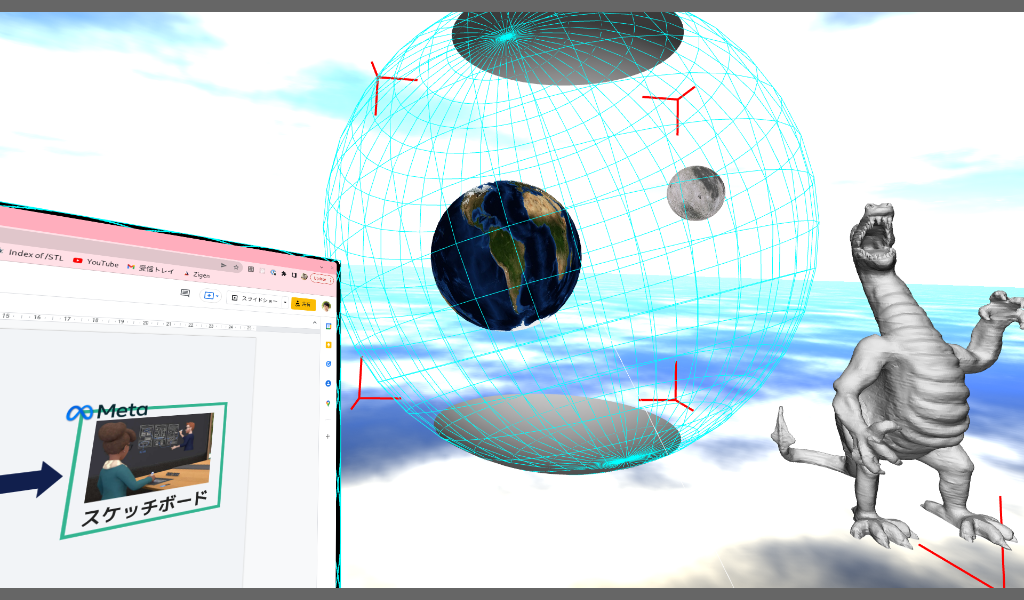
\includegraphics[keepaspectratio, width=\linewidth]{fig/multi-app.png}
    \caption{
      複数3Dアプリケーションの表示.左は既存の2Dアプリケーション(Google Chrome)
      中心はサンプルで作成した天体を表示・編集するアプリケーション,
      右は3Dファイルを表示するアプリケーション.また背景の空も1つのアプリケーションであり,
      ユーザが任意に変更可能である.
    }
    \label{fig:multi-app}
  \end{minipage}
  \begin{minipage}[t]{0.50\linewidth}
    \centering
    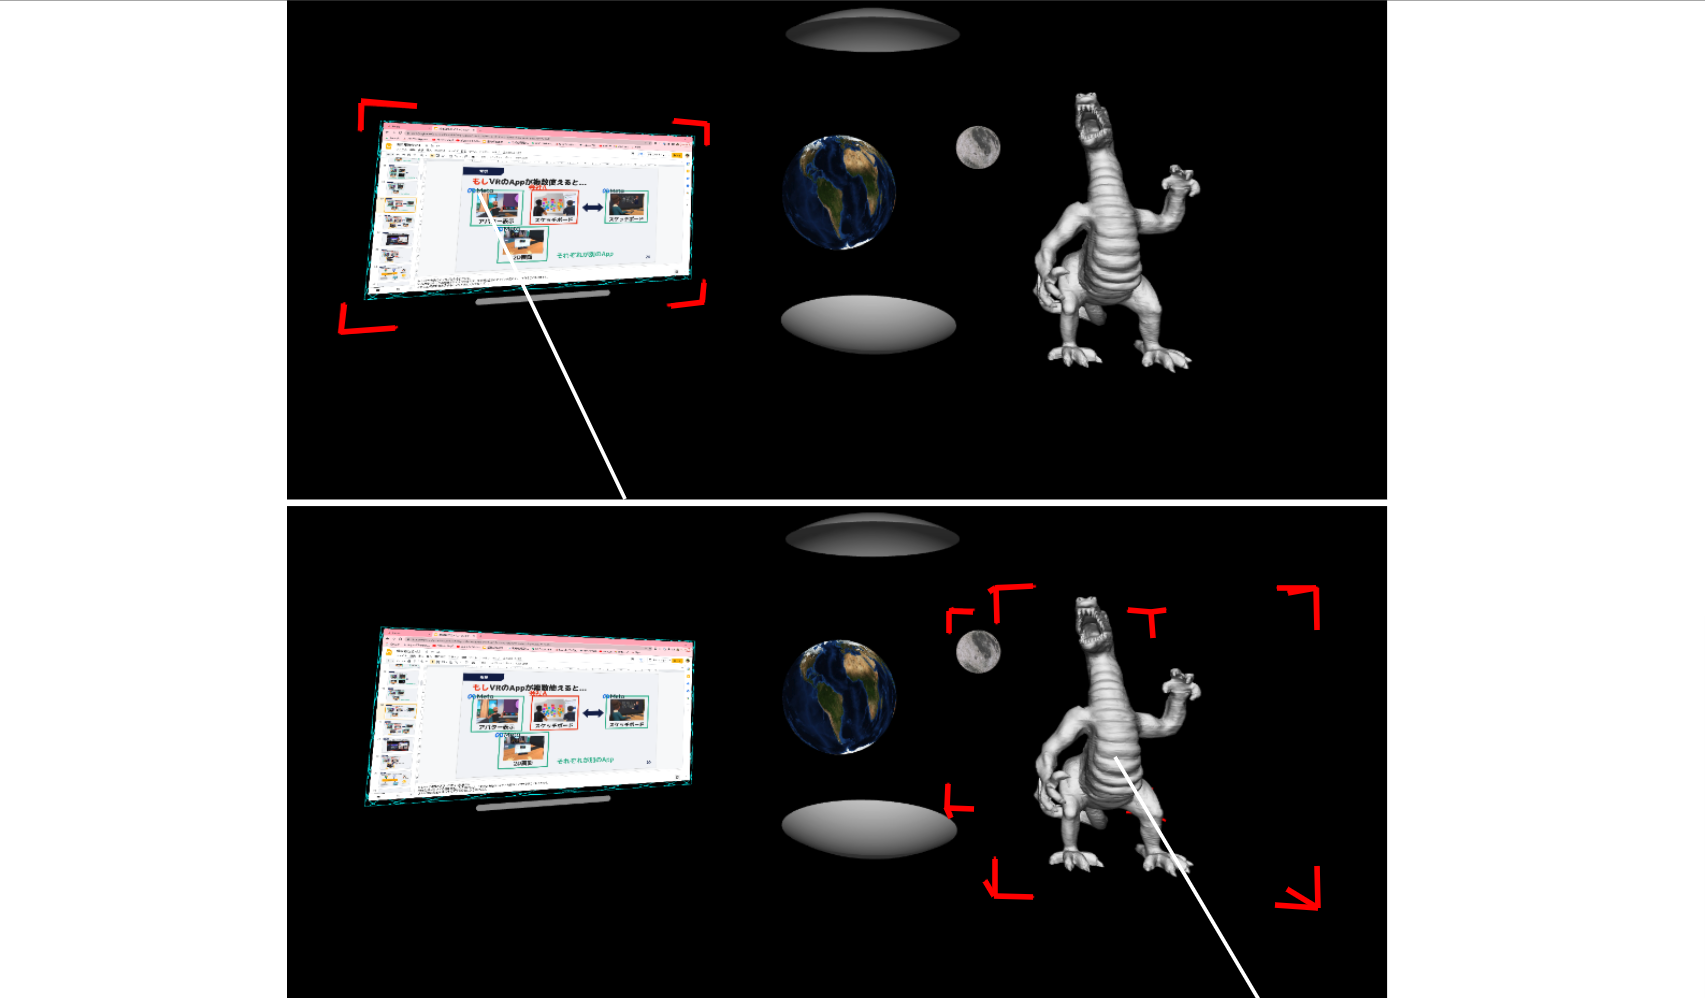
\includegraphics[keepaspectratio, width=\linewidth]{fig/ray-input.png}
    \caption{
      Rayによって3Dアプリケーションへのフォーカスを切り替えている様子.
      上段は一番左のアプリケーションに,下段は一番右のアプリケーションにフォーカスしており,
      アプリケーションがハイライトされている様子がわかる.
    }
    \label{fig:ray-input}
  \end{minipage}
\end{figure}

\begin{figure}[htbp]
  \begin{minipage}[t]{0.50\linewidth}
    \centering
    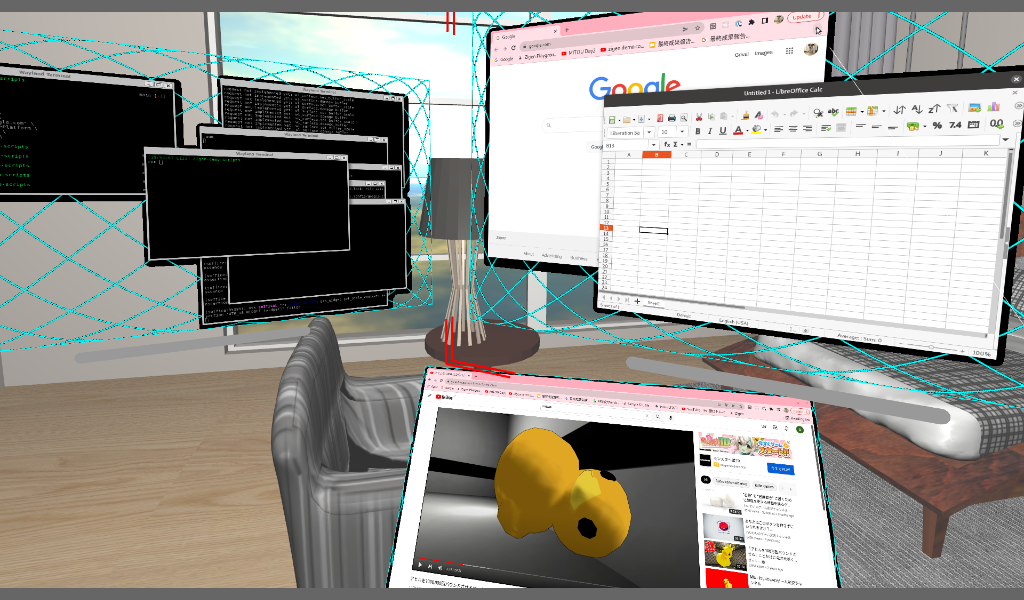
\includegraphics[keepaspectratio, width=\linewidth]{fig/2d-apps.png}
    \caption{
      ブラウザなどの既存の2Dアプリケーションが修正なしでそのまま動作する.
    }
    \label{fig:2d-apps}
  \end{minipage}
  \begin{minipage}[t]{0.50\linewidth}
    \centering
    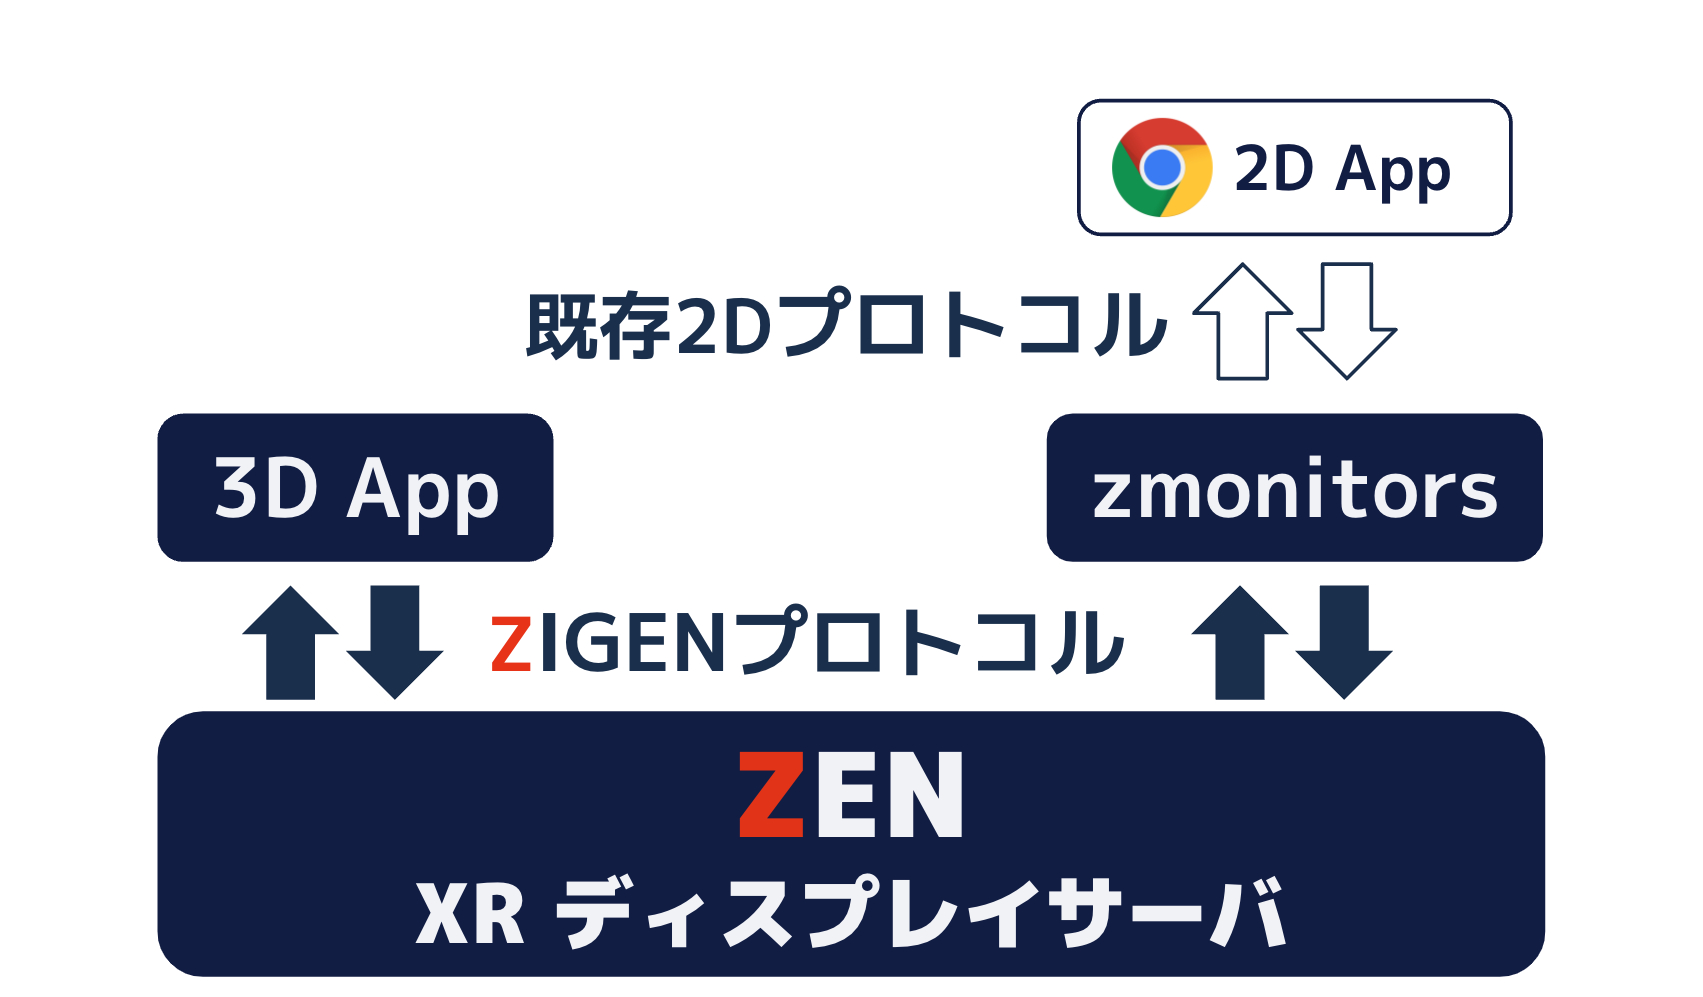
\includegraphics[keepaspectratio, width=\linewidth]{fig/zmonitors.png}
    \caption{
      既存の2Dアプリケーションを3Dアプリケーションに変換するzmonitors.
    }
    \label{fig:zmonitors}
  \end{minipage}
\end{figure}

\begin{figure}[htbp]
  \begin{minipage}[t]{0.50\linewidth}
    \centering
    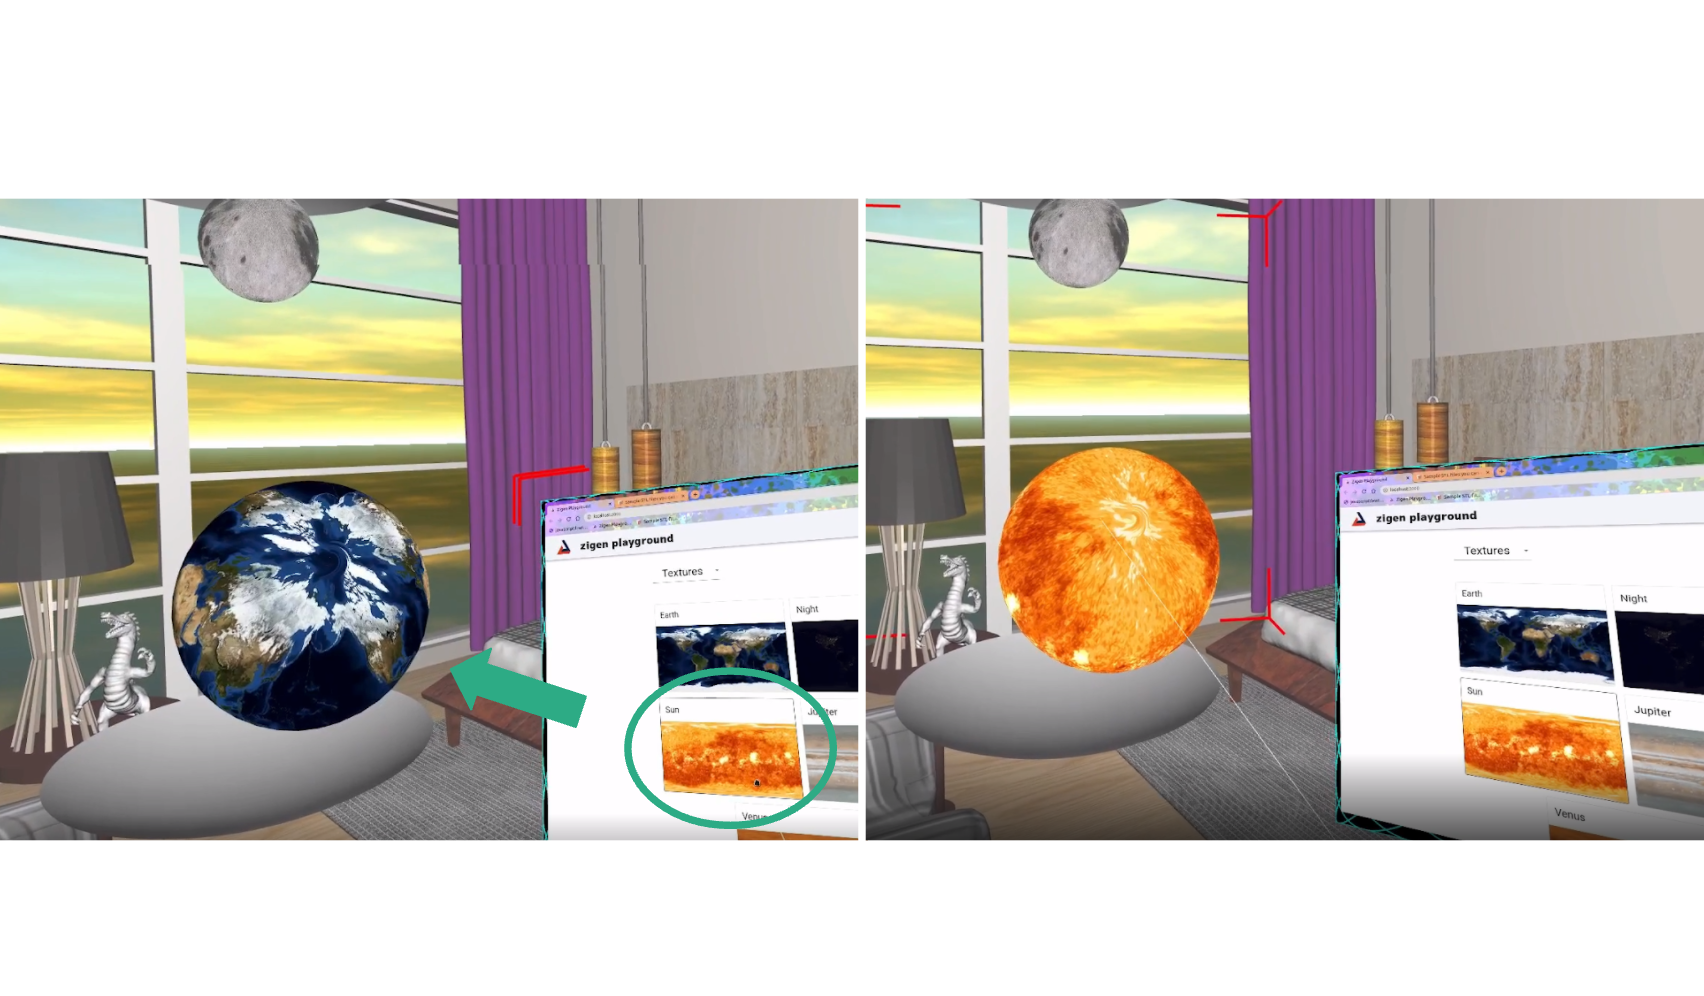
\includegraphics[keepaspectratio, width=\linewidth]{fig/dnd.png}
    \caption{
      Google Chromeから天体を表示・編集する3Dアプリケーションに,天体のテクスチャを
      ドラッグ \& ドロップすることで,天体を地球から太陽に変更する様子.
    }
    \label{fig:dnd}
  \end{minipage}
\end{figure}


\subsection{目的}
\label{section:objective}

本プロジェクトの目的はXR空間にWindowing Systemを導入することで
XR空間にマルチアプリケーション・マルチタスクの環境を提供することである.
\ref{section:current-status}で述べたように,本プロジェクトは未踏IT育成人材・発掘事業
% textlint-disable
において,メインのコンセプトについて概念実証を行ってきが,これをさらに社会へ実装するため,
% textlint-enable
未踏アドバンストでは以下のより詳細な目的を設定する.

\begin{enumerate}
  \item 実用レベルのXRデスクトップ環境を提供する.\\
        ユーザが日常で使うデスクトップ環境を
        提供するためには,単純にディスプレイサーバを実装するだけでは足りず,
        デスクトップシェルと呼ばれる部分などの実装が必要になる.
  \item ユーザと開発者からなるエコシステムを提供する.\\ %TODO: ここは伝わる言い方になってない。改善する。
        本プロジェクトが目指す世界の特徴として,XR空間全体ではなく,各機能がそれぞれ
        アプリケーションとなることで,機能ごとに市場競争が生じ,
        また開発者も特定の機能だけをうまく実装すればよいことになる.
        これによって現在より多様な機能や多様な開発者が生まれ,作業空間としてのXRは
        より洗練された空間になる.この世界の実現のため,まずは個人の開発者が空間の改善を行え,
        それをユーザに使ってもらえる仕組みを提供していく.
  \item 多くのユーザに実際に試してもらう.\\
        未踏IT人材発掘・育成事業では実際にユーザに使ってもらい,生のフィードバックを
        多くもらうまでは至らなかった.これを達成するためにはイベントの参加・開催,
        対応ハードウェア,認知度向上などに関してするべきことがある.
\end{enumerate}


\subsection{目標(開発面)}
\label{section:dev-goal}

\ref*{section:objective}の目的のうち開発に関連するものに対して,
本プロジェクトの未踏アドバンストにおける開発面での目標を述べる.
具体的な実装方針などについては\ref{section:dev-plan-detail}で述べる.

\subsubsection*{実用レベルのXRデスクトップ環境を提供する.}

\begin{itemize}
  \item \textbf{X11の2Dアプリケーションに対応する.}\\
        現状のzmonitors(\ref{section:current-status}の3. を参照)では % TODO: 3. に変わりないかCheck
        Waylandプロトコルにのみ対応している.つまり現状ZIGENではWayland対応の
        2Dアプリケーションしか動作しない.WaylandはUbuntu 21.04からはX11に変わって
        標準のWindowing Systemとなるなど,X11より新しいWindowing Systemであると
        % textlint-disable
        言えるが,現状多くのLinuxのGUIアプリケーションはX11でのみ動作し,それらの
        % textlint-enable
        アプリケーションが使えなければ実生活での作業空間としてZIGENを利用することは厳しい.
        % TODO: Check 単にXWaylandに対応するだけの話であることを言えてるか
        さらにX11の2Dアプリケーションへの対応に加えて,WineHQ\footnote{WineHQ - Run Windows applications on Linux, BSD, Solaris and macOS:\url{https://www.winehq.org/}}などを用いることで既存のWindows OS上で動作する2DアプリケーションもZIGEN上で使える可能性がある.
  \item \textbf{XR デスクトップ環境としての機能の充実する.}\\
        実用的な2D デスクトップ環境ではWIMPのパラダイムのもとアイコンのクリックによって
        アプリケーションを実行するといった機能が存在する.またショートカットキーによる
        アプリケーション一覧の表示や,フォーカスの切り替えなどは
        正確にはWindowing Systemとしては必須の機能ではないが,実用的なデスクトップ環境には
        求められる機能である.

  \item \textbf{2D Windowing Systemとの親和性を高める.}\\
        XR空間を作業環境として使ってもらう場合でも,全てがHMDを着用したXR空間内で
        完結することには,すぐにはならないと予想される.例えば,HMDが何かしらの理由で使えない場合は
        通常のディスプレイで作業することになるであろうし,作業環境を既存の
        2D デスクトップ環境に戻して,HMDをゲーム用途に使いたくなる可能性もある.
        ZIGENを通じて2D Windowing Systemを起動できるようにすれば,モニターで
        起動中の2D デスクトップ環境からXR デスクトップに移行する際に, 2D デスクトップのアプリケーションを
        そのままXR デスクトップに移すことができる.逆もまた然りでXR デスクトップから通常の2Dのデスクトップ環境に戻ることができる.
\end{itemize}

\subsubsection*{ユーザと3Dアプリケーション開発者からなるエコシステムを形成する.}

\begin{itemize}
  \item \textbf{ゲームエンジンでZIGENの3Dアプリケーションを作成できるようにする.}\\
        VRやARに興味があり,開発をしているひとの多くはUnityやUnrealといったゲームエンジンで
        開発をおこなっている.現状ではZIGEN上のアプリケーションを作成するには
        OpenGLに似たAPIを叩いて描画する必要があり,多くの開発者を巻き込める状況にない.

  \item \textbf{ZIGENのアプリケーションのストアを展開する.}\\
        開発者が自分が作ったアプリケーションを出品し,ユーザが自分の欲しいアプリケーションを
        検索してインストールできるストアを運営することにより,ユーザと開発者とを繋ぐハブとして
        エコシステムの活性化を図る.
        しかし,これはかなり応用的な話で,未踏アドバンストにおいてできるかはわからないが,
        継続的な開発のための収益化にもつながりうるため,視野にいれている.
\end{itemize}

\subsubsection*{多くのユーザに使ってもらう.}

\begin{itemize}
  \item \textbf{より多くのHMDへの対応}\\
        より多くのユーザに使ってもらうために,サポートするデバイスを増やす.
        特にOculus Quest2の販売台数は他の全VRヘッドセットの販売台数を上回るとも
        言われており,対応することでより多くのユーザに使ってもらう機会を増やすことができると
        考えている.

  \item \textbf{既存のXRアプリケーションと一緒に使えるようにオーバーレイとして実装する.}\\
        現在でもVRChatなど特定のXRアプリケーションを常時使い続けている人は多い.
        このような人たちをユーザとして取り込むために,他のXRアプリケーションに対して
        オーバーレイとしてZIGENの環境を使えるようにすることで,VRChatでコミュニケーションを
        とりながら,よりよい個人の作業空間を展開するなどといったことができるようになる.
\end{itemize}

\subsection{目標(社会実装面)}

\ref{section:objective}の目的のうち社会実装に関連するものに対して,
本プロジェクトの未踏アドバンストにおける社会実装面での目標を述べる.
% 具体的な施策に関しては\ref{section:biz-plan-detail}で述べる.

ここで事業性の面で本プロジェクトが主に目指すところは,収益化ではなく,
現状のXRにおける課題を解決し,作業空間としてのXRのあるべき世界を指し示し,
社会にインストールすることである.ただし,プロジェクトの継続的な発展や開発母体の安定性のために,
収益化の方法を模索することは必要であると思っており,未踏アドバンスト事業期間中にそのための
検証などを行なっていくつもりである.

\subsubsection*{ユーザと3Dアプリケーション開発者からなるエコシステムを形成する.}

% \item 開発者ドキュメントを整備する.
まずは開発や利用に関して気軽に質問などができるコミュニティを目指し,
Discordなどのコミュニティツールの整備や,その広報をおこなっていく.
ターゲットユーザの近い類似プロジェクトの現状を鑑みて以下の目標数値を定める.

\begin{itemize}
  \item Discordユーザ:300人 (現状36人)
  \item 外部からのIssue/PullRequest:5つ
\end{itemize}

また,外部の開発者に実際にアプリケーションを作ってもらい試してもらうためのハッカソンを
開催する.

\subsubsection*{多くのユーザに使ってもらう.}

幅広い知識レベルのユーザが利用できるようにインストラクションドキュメントを提供すると共に,
カンファレンスやイベント,メディアへの露出や,ブログによる情報発信を通して認知度の向上を図る.

\subsubsection*{XR世界を作り上げているコミュニティでのプレゼンスを高める.}

OSSとしてのコミュニティの完成度を高めるため.
GitHubが提供しているOSSプロジェクトのガイドライン
\footnote{オープンソースガイドライン:https://opensource.guide/ja/}
を実践する.
また,先に述べたカンファレンスやイベントなどの登壇もプレゼンスの向上に寄与すると考える.

\subsubsection*{事業の継続のための収益化について.}

開発継続のための金銭を受け取る方法はいくつか模索している.

\begin{itemize}
  \item \textbf{助成金やクラウドファウンディングなどで金銭を得る\\}
        OSS向けのFoundationは多く存在するが,その中でも特に
        XR Foundation\footnote{XR Foundation:https://www.xrfoundation.io/}や,
        Open 3D Foundation\footnote{Open 3D Foundation:https://o3d.foundation/}
        などのXR向けのFoundationに絞って申請を検討する.また,Webpack\footnote{Webpack:https://webpack.js.org/}などはOpenCollective
        \footnote{webpack - OpenCollective https://opencollective.com/webpack}
        を通じて企業や個人から資金を得ていたり,Kickstarterのキャンペーンを通じてDjangoの
        スキーママイグレーションの活動資金を得ているプロジェクト
        \footnote{https://www.kickstarter.com/projects/andrewgodwin/schema-migrations-for-django}
        なども存在する.
  \item \textbf{ビジネスとして展開する.\\}
        ZIGENにおいてビジネス展開を考える場合はHMDやLinux PCを持っている人の絶対数が
        多くはないためそこが難しい.そのため,ZIGENをセットアップした状態のハードウェア
        含めたXR作業環境一式,またはその一部(HMDとWindowing Systemのみなど)
        を法人向けに提供することを考えている.昨今はクラウドサービスが増え,
        Google SheetのようにOSに依存せず,ブラウザさえあれば仕事が完結する場合も
        多くなってきており,Linuxのデスクトップ環境でも十分に仕事が可能になってきている.
        とくにエンジニア向けにエンジニアを抱える法人に対してアプローチしていきたい.
\end{itemize}

未踏アドバンスト事業期間での目標は,助成金またはクラウドファンディングなどにはいずれか1つ以上
申請し,ビジネス展開については普段から仕事でLinuxを使っている開発者,そうでない開発者,
非開発者などの属性それぞれに対して,ZIGENでの作業環境に移行する可能性があるか
% textlint-disable
ユーザインタビューを行い検証していきたい.
% textlint-enable

% TODO: 収益化に関するetc


\subsection{他プロジェクトとの差分}

\subsubsection{xrdesktop / wxrd}

xrdesktopはLinuxの2Dデスクトップ環境をXR空間から操作することを実現するプロジェクトである
(図\ref{fig:xrdesktop}).Google が主催する OSS 人材育成プロジェクトである
Google Summer of CodeにもOSSプロジェクト側で出るほど信頼度の高いOSSプロジェクトである.
既存の2Dアプリケーションが動作する点はZIGENと同じだが,
アプリケーションがXR空間に3Dのオブジェクトを表示することなどは視野にない.
また,GNOMEやKwinといった既存のデスクトップ環境のウィンドウのミラーを表示するという
実装であるため,ウィンドウのリサイズや移動などを通常の2Dデスクトップ環境と同じように
行うことはできていない.ZIGENが始動した時期と同時期の2021年7月から
同じ開発者が"wxrd"という同様の機能をWaylandコンポジッタを用いて提供するプロジェクトを
試験的に始めており,これはZIGENが2Dアプリケーションを表示している仕組みと近い設計で,
HMDのリフレッシュレートに合わせられていなかった問題などを解消できるとしている
(ZIGENは実現できている).xrdesktop以外にもLinuxに限らず2Dのデスクトップ環境を表示する
機能であれば,商業的にも数多く存在する.しかしいずれにせよ複数の3Dアプリケーションを立ち上げる
環境はない.

\begin{figure}[htbp]
  \begin{minipage}[t]{0.50\linewidth}
    \centering
    
\includegraphics[keepaspectratio, width=\linewidth]{fig/xrdesktop.png}
    \caption{xrdesktop.}
    \label{fig:xrdesktop}
  \end{minipage}
\end{figure}

\subsubsection{OpenXR Overlay}
\label{section:openxr-overlay}

OpenXRとは,ベンダに依存しない統一的なXRプラットフォームやデバイスのインタフェースを提供する
もので,Khronos グループによって策定されており,XRプラットフォーム・デバイス標準化の
デファクトスタンダードになりつつある.
OpenXRの定義の中にはOverlayという仕組みがあり,メインのアプリケーションの上に重ねて
他のアプリケーションを表示できる.またこの合成時にはDepthテストを行うこともできるので,
3Dアプリケーションどうしは前後関係含めて自然に合成して表示できる.

しかしこれは単純にアプリケーションを重ねて表示するだけであり,
複数のアプリケーションがユーザの入力を衝突せずに受け取る仕組みや,
アプリケーション間でのドラッグ \& ドロップのようなベンダに依存しないデータ共有の仕組みは
存在しない.そのため,Overlayのアプリケーションを複数起動して,それらを連携して使うような
使い方には至っていない.

しかしZIGENでは入力の割り振りやデータ共有の仕組みがあるため,マルチアプリケーション・
マルチタスクの環境を提供できる.

\subsubsection{
  Toward General Purpose 3D User Interfaces:
  Extending Windowing Systems to Three Dimensions \cite{forrest}
}
\label{section:forrest}

これはForrestによる2014年の修士論文である.
この論文では,3D没入環境にマルチアプリケーションの環境を提供し,また(当時)XRにおいて
ハードウェアが乱立していてその共通インタフェースがない問題を解決するため,
Windowing Systemを3Dに拡張することを提案し,その場合のウィンドウに相当する概念や,
ハードウェアの抽象化,アプリケーションの描画情報の受け渡し方などについて考察している.

本プロジェクトとの差分としては,実際にユーザが使える状態まで実装される予定がないこと,
ドラッグ \& ドロップなどのデータ共有の仕組みについて言及されていないこと,
その他アプリケーションの描画情報の送り方やアプリケーションの移動などの操作など
細かい部分まで含めると多くあるが,達成したいことはかなり似ており,
Cuboid Windowと呼ばれる概念などはZIGENにも取り入れたりなど,
大変参考にしている論文である.


% 提案の背景、目的、目標を、開発と事業化(または社会課題の解決に寄与するような社会実装)の
% 両面について、その分野の専門家でない人にもわかるように丁寧に記述してください。
% また、競合する事業等が存在する場合には、その概要及び競合との差別化要因になるものについて、
% 記載してください。

% 提案の背景(なぜ)、目的(なにを)、目標(どこまで)を、
% 開発と事業化(または社会課題の解決に寄与するような社会実装)の両面で記載
% 競合する事業等が存在する場合には、その概要及び競合との差別化要因
